\documentclass{article}

% if you need to pass options to natbib, use, e.g.:
%     \PassOptionsToPackage{numbers, compress}{natbib}
% before loading neurips_2019

% ready for submission
% \usepackage{neurips_2019}

% to compile a preprint version, e.g., for submission to arXiv, add add the
% [preprint] option:
%     \usepackage[preprint]{neurips_2019}

% to compile a camera-ready version, add the [final] option, e.g.:
     \usepackage[final]{mlcb_2019}

% to avoid loading the natbib package, add option nonatbib:
%     \usepackage[nonatbib]{neurips_2019}

\usepackage[utf8]{inputenc} % allow utf-8 input
\usepackage[T1]{fontenc}    % use 8-bit T1 fonts
\usepackage{hyperref}       % hyperlinks
\usepackage{url}            % simple URL typesetting
\usepackage{booktabs}       % professional-quality tables
\usepackage{amsfonts}       % blackboard math symbols
\usepackage{nicefrac}       % compact symbols for 1/2, etc.
\usepackage{microtype}
\usepackage{amsmath}      % microtypography
\usepackage{bm}
\usepackage{graphicx}
\usepackage{verbatim}
\usepackage{wrapfig}

\title{End-to-end RNA Secondary Structure Prediction using Deep Neural Network}

% The \author macro works with any number of authors. There are two commands
% used to separate the names and addresses of multiple authors: \And and \AND.
%
% Using \And between authors leaves it to LaTeX to determine where to break the
% lines. Using \AND forces a line break at that point. So, if LaTeX puts 3 of 4
% authors names on the first line, and the last on the second line, try using
% \AND instead of \And before the third author name.

% double-blind
%\author{%
%  TODO \\
%  Department of Electrical and Computer Engineering\\
%  University of Toronto\\
%  \texttt{todo@toronto.edu} \\
%  % examples of more authors
%  % \And
%  % Coauthor \\
%  % Affiliation \\
%  % Address \\
%  % \texttt{email} \\
%  % \AND
%  % Coauthor \\
%  % Affiliation \\
%  % Address \\
%  % \texttt{email} \\
%  % \And
%  % Coauthor \\
%  % Affiliation \\
%  % Address \\
%  % \texttt{email} \\
%  % \And
%  % Coauthor \\
%  % Affiliation \\
%  % Address \\
%  % \texttt{email} \\
%}

\begin{document}

\maketitle

%\begin{abstract}
%  TODO
%\end{abstract}

\vspace*{-7em}

\section{Introduction}

%Once believed to be an intermediate molecule that serves as a messenger between DNA and protein,
%RNA is now known to be involved in many aspects in gene regulation and expression.
Unlike DNA which typically forms stable double helix between two molecules, RNA is highly flexible
such that a single RNA molecule can fold onto itself by
forming base pairs via hydrogen bonds, including Watson-Crick pairs A-U,
G-C and non-canonical pairs such as G-U.
Base pairs form local structures like stems and loops,
which assemble into the global secondary structure.
%These base pairs act as building blocks, from which local structure forms? global?

State-of-the-art RNA secondary structure prediction algorithms,
such as ViennaRNA\cite{lorenz2011viennarna} and Mfold\cite{zuker2003mfold},
are based thermodynamics.
Each type of local structure comes with free energy that is measured experimentally,
and total free energy is assumed to be the sum of all local free energy,
which is minimized efficiently using dynamic programming.
Although researchers have worked out a large set of local structure types and
their associated formulation for free energy calculation,
there is no guarantee that it's either accurate or complete.
There has been effort to fine tune the free energy parameters by
training on experimentally solved structures\cite{andronescu2007efficient},
but it's still limited by the known set of local structure types.
Another limitation of dynamic programming based approaches is that
it is incapable of predicting nested base pairs that appear in structure like pseudoknot.


%Moreover, over the last decade,
%combination of RNA structure probing and high throughput sequencing has enabled
%the measurement of genome-wide RNA structural at single nucleotide resolution in multiple organisms and cell types,
%which have only been combined? with dynamic programming using heuristics (ref?).
%Such data also exhibit a high level of noise and sometimes with missing data (ref, sequencing, DMS),
%which also calls for new approaches that can be trained end-to-end on different types of data,
%to model ?differences in cell types and conditions.

Moreover, over the last decade,
combination of RNA structure probing and high throughput sequencing has enabled
the measurement of genome-wide RNA structural at single nucleotide resolution in multiple organisms and cell types (TODO citation).
Due to the level of noise and missing data present in high throughput experiments,
we will need a modelling approach that is more flexible and can be trained on different types of data.
%Such data can be valuable in learning cell type specific RNA secondary structure model,
%
%Such data also exhibit a high level of noise and sometimes with missing data (ref, sequencing, DMS),
%which also calls for new approaches that can be trained end-to-end on different types of data,
%to model ?differences in cell types and conditions.

In this work, we propose a deep neural network that can be trained end-to-end on
sequences and structures. When conditioned on the input RNA sequence,
the model can generate a distribution of structures, including ones with pseudoknot.
%We start by describing the problem formulation, followed by a brief review of
%related work, and present the model
%differentiable

%TODO if we mention the above we'll need to talk about how to train on those data.
%
%sequence alone
%
%one sequence, many structures

\subsection{Problem Formulation}

Given a RNA sequence of length $L$, we are interested in all possible secondary structures it can take on.
%There are three common ways to represent a specific RNA secondary structure:
For a specific structure, there are three common ways to represent it:
(1) Undirected graph, where each node is a base in the sequence, and each vertex represents base pairing.
(2) Upper triangular matrix (excluding the diagonal)
of size $L \times L$ with binary values, where a value of $1$ at $(i, j)$ represents
base pairing between sequence position $i$ and $j$, and $0$ represents no base paring.
(3) Dot-bracket notation of length $L$ where unpaired based are denoted as dots,
    and paired bases are represented as left and right brackets.
When pseudoknot is present, different styles of bracket needs to be used to represent nested structures.


%\begin{itemize}
%
%    \item Undirected graph, where each node is a base in the sequence, and each vertex represent base pairing.
%
%    \item Upper triangular matrix (excluding the diagonal)
%of size $L \times L$ with binary values, where a value of $1$ at $(i, j)$ represents
%base pairing between sequence position $i$ and $j$, and $0$ represents no base paring.
%
%    \item A dot-bracket notation of length $L$ where unpaired based are denoted as dots,
%    and paired bases are represented as left and right brackets.
%
%\end{itemize}

As an example, for a short RNA sequence GUUGUGAAAU, one possible structure it can take on
%(Entry \verb|CRW_00083| from \cite{andronescu2008rna})   # TODO this entry nmumber is not correct!
%takes a structure that
consists of a stem and a loop, as seen in Fig \ref{fig:rna_ss_binary_mat}(a), represented by an undirected graph.
Such structure can also be represented by an upper triangular $10 \times 10$ matrix with all $0$'s,
except for positions
%$y_{1, 10}, y_{2, 9}$ and $y_{3, 8}$,
$(1, 10), (2, 9)$ and $(3, 8)$,
all being $1$, as shown in Fig \ref{fig:rna_ss_binary_mat}(b).
This contiguous stretch of $1$'s along the diagonal corresponds to the stem formed by the three base pairs: G-U, U-A and U-A.
The equivalent dot-bracket notation is shown in Fig \ref{fig:rna_ss_binary_mat}(c), where the three pairs
of left-right brackets represent the stem.
%(TODO define x and y first)


\begin{wrapfigure}{R}
%    \begin{figure}[h]
        \centering
        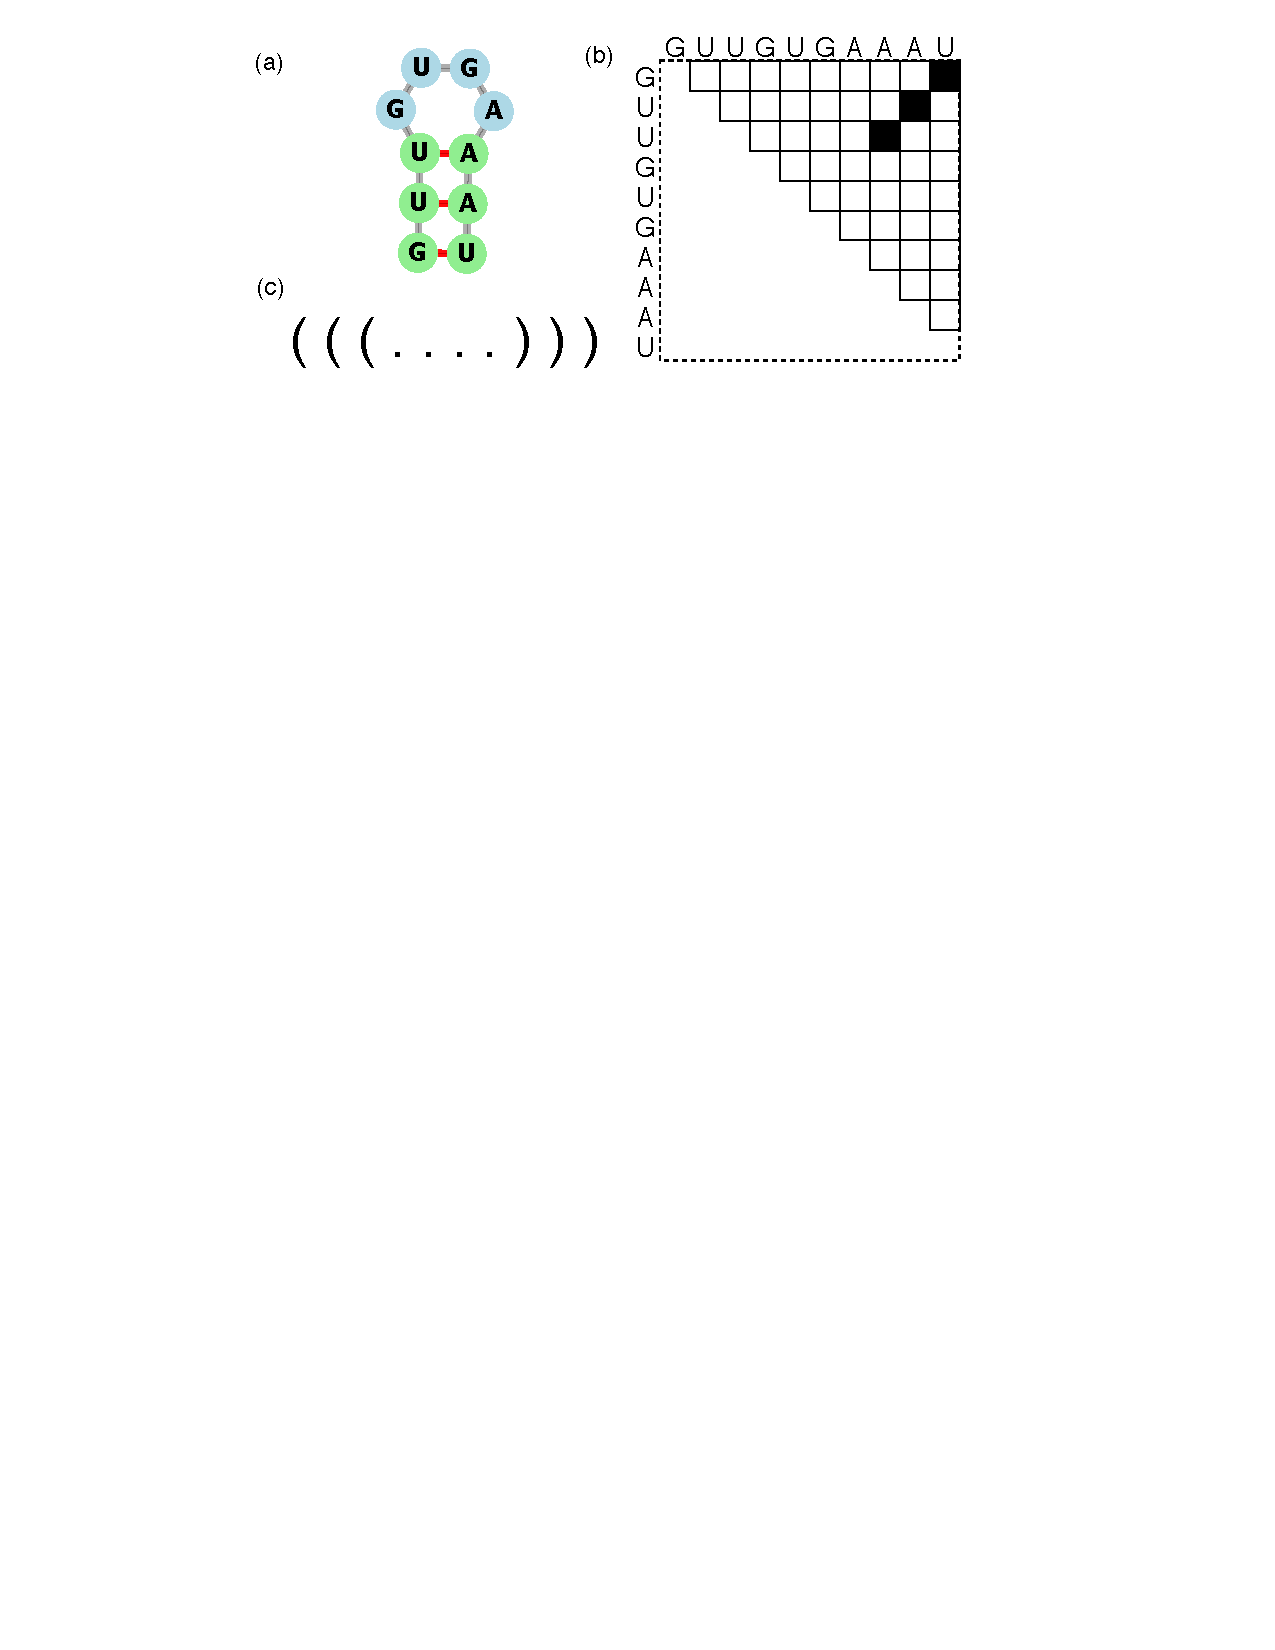
\includegraphics[width=0.4\textwidth]{plot/rna_ss_binary_mat.pdf}
        \caption{Three different ways to represent secondary structure of the RNA sequence GUUGUGAAAU. (a) undirected graph, generated by \cite{kerpedjiev2015forna}, (b) upper triangular binary matrix, (c) dot-bracket notation.}
        \label{fig:rna_ss_binary_mat}
        \centering
%    \end{figure}
\end{wrapfigure}

%\begin{wrapfigure}{R}
%%    \begin{figure}[h]
%        \centering
%        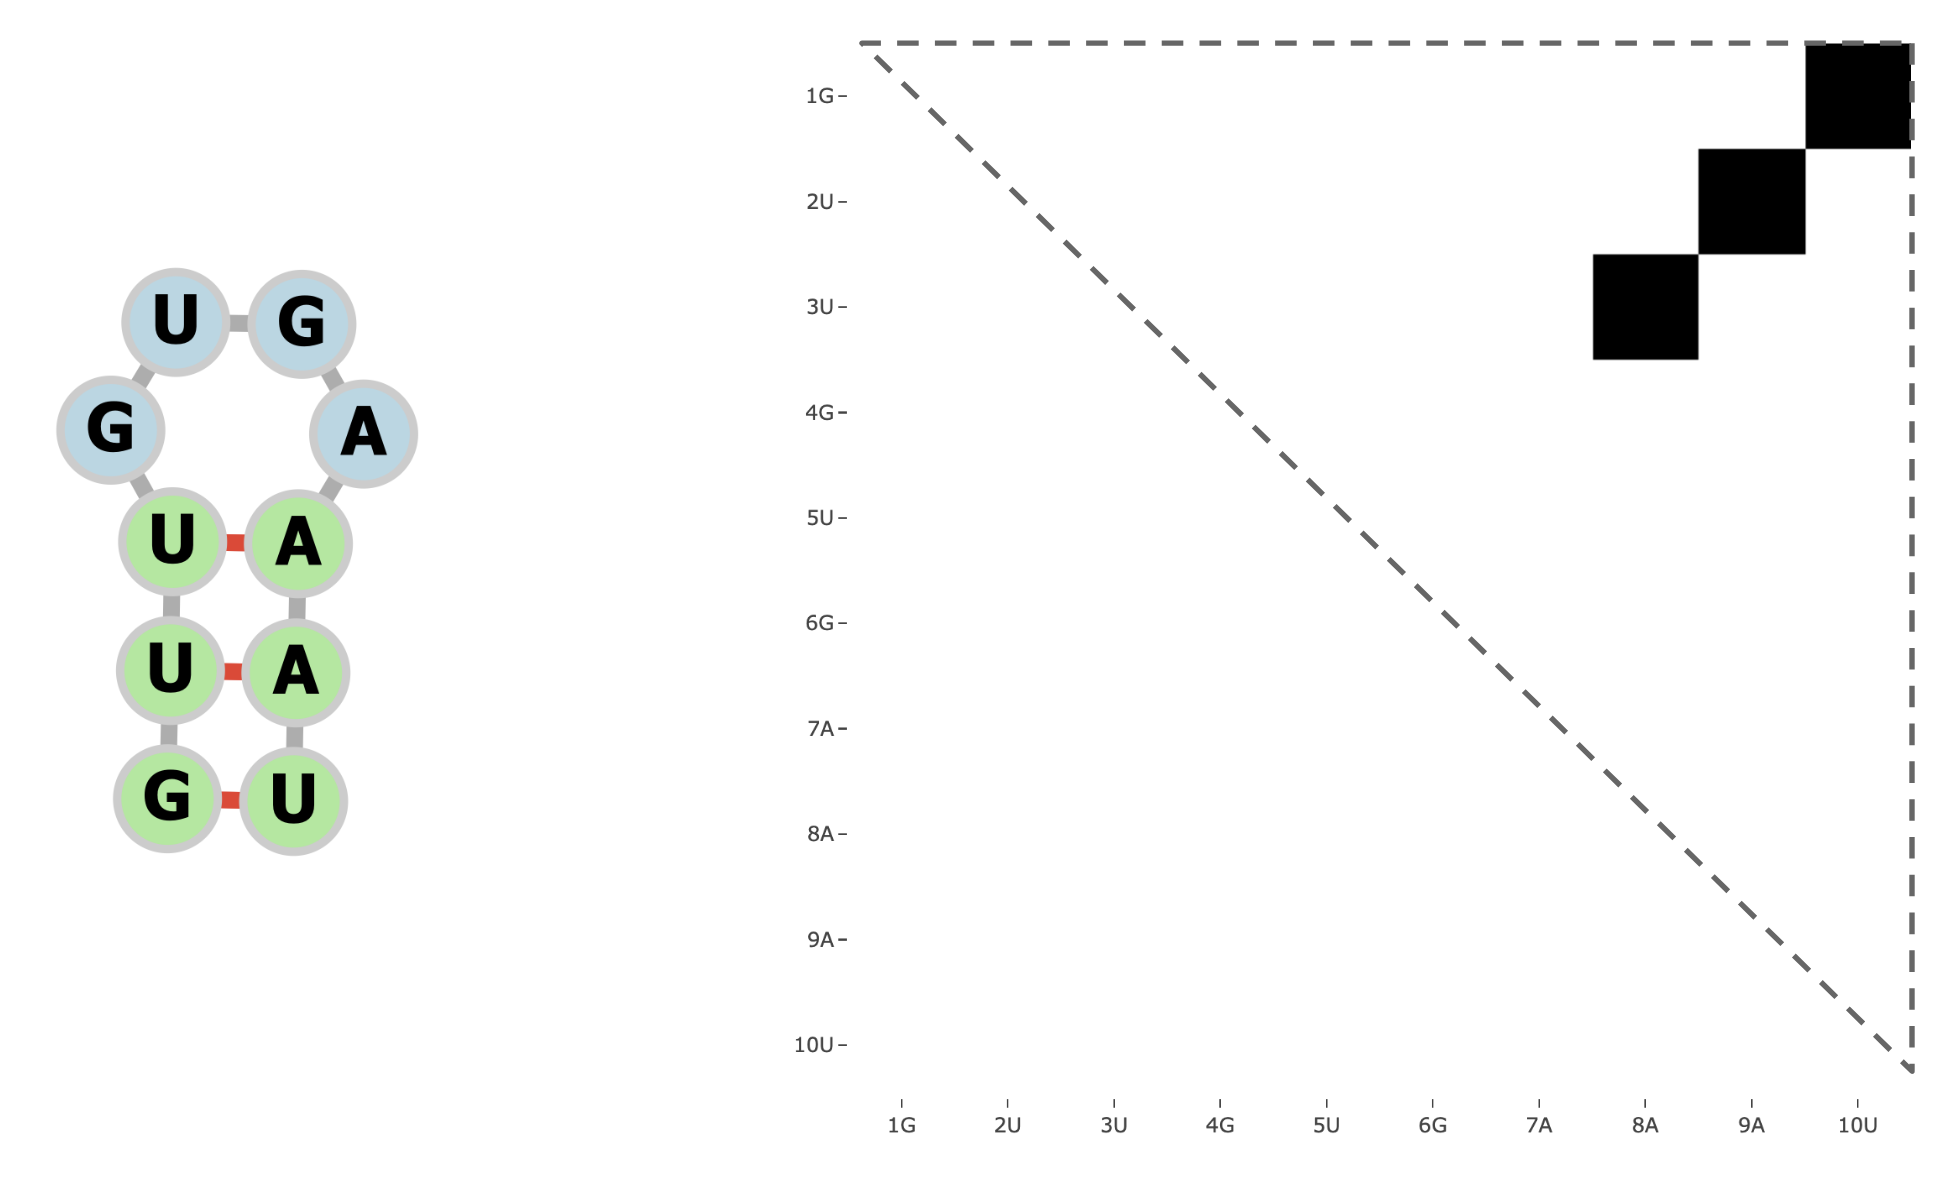
\includegraphics[width=0.5\textwidth]{plot/rna_ss_binary_mat.png}
%        \caption{TODO}
%        \label{fig:rna_ss_binary_mat}
%        \centering
%%    \end{figure}
%\end{wrapfigure}



%TODO maybe talk about pairing matrix and dot-bracket notation here, to make it easier for literature review.

\subsection{Related Work}

There have been a few work that solve partial problem....

Wu\cite{wu2018convolutional} presented a convolution neural network to predict the free energy of local structure motifs.
Convolution was run on circular matrix representation of the structure motif, to reflect the loop-like nature of local structures.
%Circular convolution was proposed as a nature fit for loop-like structures.
The model was trained on experimentally measured free energy of short structure motifs,
as well as random structure motifs whose energy was estimated using existing linear approximation models.
Although it shows promising result on modelling free energy of short structure motif from experimental data,
and can be used to estimate the free energy for a \textit{given} structure,
it does not solve the problem of predicting structure from sequence.

Other work were done to tackle the learning problem end-to-end.
Researchers have framed the problem as a sequence to sequence learning task,
and the proposed model either predicts the probability of being paired for each base,
or some forms of the dot-bracket notation.
Willmott et. al\cite{willmottstate} proposed a bidirectional LSTM that predicts
from RNA sequence the probability for 3 classes: paired, unpaired, and end-of-Sequence.
The model was trained on experimentally solved structure of 16S rRNAs.
It it unclear whether the model generalize to other types of RNAs.
Zhang et. al\cite{zhang2019new} proposed using convolutional neural network to predict from sequence
the dot-bracket notation, where each position is encoded as a 3-class softmax: left bracket, right bracket and dot.
In order for a dot-bracket notation to yield valid structure, it has to follow a few syntactic constraints.
For example, each left bracket needs to have a corresponding right bracket.
As the authors have mentioned in the paper, output produces by the neural network
is not guaranteed to be valid, thus needs to be further processed by dynamic programming
to yield a valid structure prediction.
Wang et. al\cite{wang2019dmfold} used bidirectional LSTM and modelled the dot-bracket notation as a
7-class softmax, which also includes additional bracket notations to allow for pseudoknots.
Similar to \cite{zhang2019new}, the prediction does not yield a valid structure, and needs to be corrected by additional logic.
Furthermore, they used a dataset consisting of only four RNA families,
but reported performance based on randomized training and validation set split.
Random split is almost certain to result in sequences from the same family to be in both the training and validation set,
thus the generalization performance of the model remains unclear.
%he model was trained on only ? RNA families, and CV split was random,
%so generalization performance is unclear.



Existing work either solves a partial problem, or attempts at modelling the problem end-to-end,
but requires complicated post-processing to yield valid structure prediction.
In this work, we propose a novel method to model the sequence to structure predictive task end-to-end, with
no additional post-processing.



%RNA Secondary Structure Prediction by MFT Neural Networks
%\cite{apolloni2003rna}

%A New Method of RNA Secondary Structure Prediction Based on Convolutional Neural Network and Dynamic Programming
%\cite{zhang2019new}

%Convolutional models of RNA energetics
%\cite{wu2018convolutional}

%Recurrent Neural Networks and Their Applications to RNA Secondary Structure Inference
%\cite{willmott2018recurrent}

%RNA Secondary Structure Prediction Using Neural Machine Translation
%\cite{zhang2016rna}

%State inference of RNA secondary structures with deep recurrent neural networks  (replace above thesis)
%\cite{willmottstate}

%SCFG: Learning RNA secondary structure (only) from structure probing data
%not that relevant, maybe we can skip it
%
%TODO talk about what's lacking in all above approaches.


%\begin{itemize}
%
%    \item State-of-the-art methods based on dynamic programming.
%Basic building blocks are known local structure, with their associated free energy measured experimentally.
%Fixed energy parameters and hand-crafted rules.
%
%    \item Emerging new dataset calls for flexible, extensible,
%    end-to-end model that can be trained on new types of dataset (noisy, missing value).
%
%    \item TODO review other papers using NN and discuss what's lacking.
%
%\end{itemize}

%notation: we use ??? to represent a binary upper triangular matrix of size LxL.

\section{Method}


In this work, we propose a deep neural network that can be trained end-to-end on dataset with sequences and structures.
The model is capable of generating a distribution of structures, including structure with pseudoknot,
conditioned on the input sequence.

We formulate the predictive task as a conditional generative process.
Specifically, given an input sequence with arbitrary length $L$: $\bm{x} = x_1, x_2, \dots x_{L}$,
we want to predict a distribution of structures conditioned on the sequence $P(\bm{Y} \mid \bm{x})$,
where the structure $\bm{Y}$ is represented by an upper triangular matrix of size $L \times L$, as defined in Fig \ref{fig:rna_ss_binary_mat}(b).

%(TODO use the above notation).

%(move the following paragraph to the model section)
We factorize the conditional distribution as follows:
%In this work, we pick a specific way to factorize the conditional distribution,

\begin{equation} \label{eq:conditional_distribution}
P(\bm{Y} \mid \bm{x}) = P(\{y_{i, i+1}\}_{i=1, 2, \dots L-1} \mid \bm{x})
P(\{y_{i, i+2}\}_{i=1, 2, \dots L-2} \mid \bm{x}, \{y_{i, i+1}\}_{i=1, 2, \dots L-1})
\dots
P(y_{1, L} \mid \bm{x}, \{y_{i, j}\}^{i \neq 1}_{j \neq L})
\end{equation}

%which mimcs the autoregressive process, where the time axis in our case is the distance to the off-diagonal line.

The generative process implied by such formulation is illustrated in Fig \ref{fig:autoregressive_direction}.
We generate one off diagonal slice at a time, conditioned on the input sequence and the previous slices,
starting from the one adjacent to the diagonal line, shown in light blue with $t=1$.
This process continues until we fill the upper triangular matrix,
where the last entry (dark blue, shown with $t=9$) is generated conditioned on the input and the entire upper triangular matrix except for itself.
Intuitively, the distance to the off-diagonal line is the "timestamp" as in traditional autoregressive models.

%TODO re-generate plot using draw.io, or use the model plot?
%
%We generate one off diagonal slice at a time, conditioned on the input sequence and the previous slices,
%starting from the one adjacent to the diagonal line, as shown in yellow on the plot.
%When generating the second slice (in green), we condition on the input sequence and the generated values in the first slice (in yellow).
%When generating the third one (in blue), we condition on the input sequence and both the yellow and green slices.
%This process continues until we fill the upper triangular matrix,
%where the last entry (in red TODO color plot) is generated conditioned on the input and the entire upper triangular matrix except for itself.
%
%Above paragraph is quite long, cut it?

\begin{wrapfigure}{R}
    \centering
    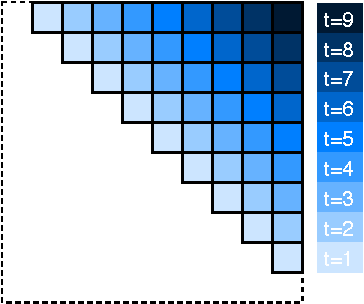
\includegraphics[width=0.3\textwidth]{plot/autoregressive_direction.pdf}
    \caption{Generative process implied by factorization of the conditional distribution in Equation \ref{eq:conditional_distribution}.}
    \label{fig:autoregressive_direction}
    \centering
\end{wrapfigure}

%TODO make sure timestamp in the other plot match with this one

%intuition, sample local connectivity then global?


\subsection{Model}

%(TODO doesn't flow well, combine with previous paragraphs?)

We propose an architecture that builds global structure from local interactions between all positions on the sequence,
without having any assumptions of the types of local structure and hard-coded parameters,
such that the entire model can be trained end-to-end using only sequences and structures.
The architecture consists of the following components:

\begin{wrapfigure}{R}
%    \begin{figure}[h]
        \centering
        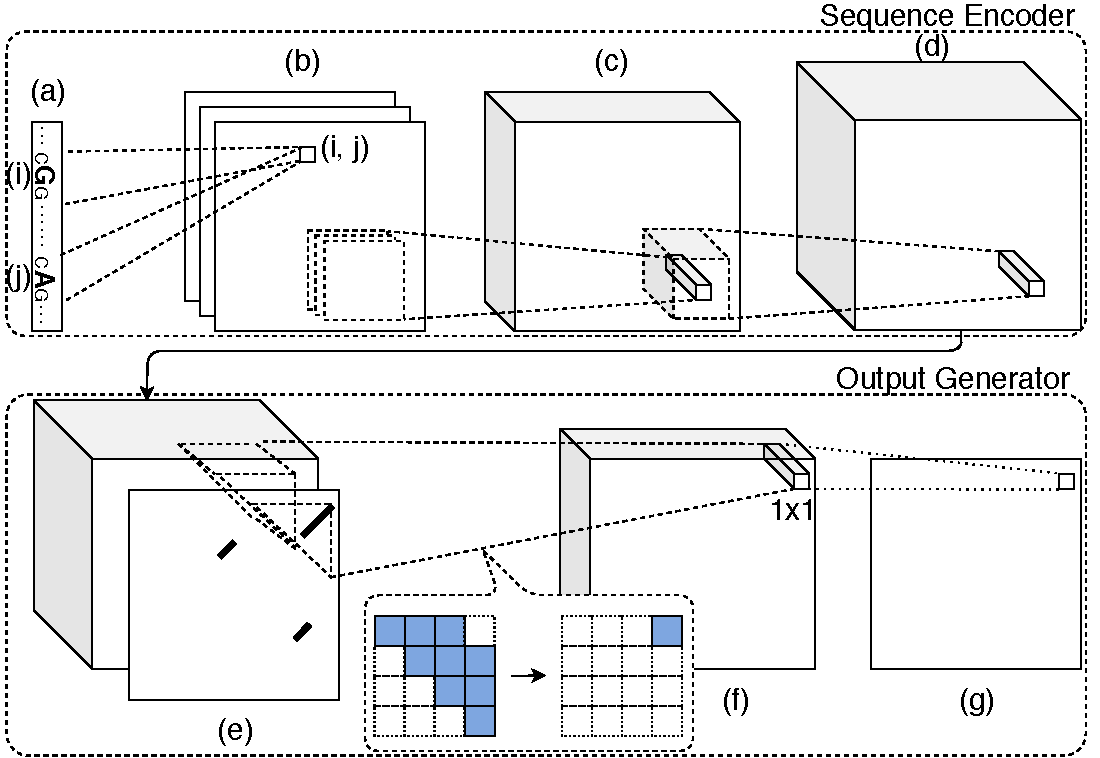
\includegraphics[width=0.6\textwidth]{plot/nn_arch_1.pdf}
        \caption{Proposed model architecture. Top: sequence encoding. Bottom: generate structure.}
        \label{fig:nn_arch_1}
        \centering
%    \end{figure}
\end{wrapfigure}


%Incoporate biological knowledge.

%TODO refer to parts in plot when talking about architecture.
%
%TODO itemize takes a lot of space, trim it? or combine items.
%gorup things so they bettwen correspond to stuff on the plot.

%TODO label plot to make it easier to refer to different components

\begin{itemize}

    \item Two sets of 1D convolution layers on the 1-hot-encoded sequence are run in parallel,
     each set has multiple convolution layers at different resolutions.
%    Note that although not shown explicitly on the plot (to keep it simple), multiple 1D conv layers...stacked...

    \item Activations of each 1d conv layer, one from each set, are used to form a 2D feature map,
where the (i, j)-th entry is the dot-product (can be replaced by a fully connected NN) between the
activation of first set at position $i$, and the activation of second set at position $j$.
This is illustrated in Fig \ref{fig:nn_arch_1}.
%    \item where the ? shows one element at position $(i, j)$ in one
%2D feature map is created by the dot-product between the
%two sets of activation units of a specific 1D convolution layer (in this case the first one)
%at position $i$ and $j$.
The idea of such set up is inspired by the fact that whether two bases form base pair or not
is not only affected by the two nucleotides but also surrounding sequences.
Such architecture can enable the neural network to learn low level sequence features that affect the 'compatibility'
between two stretches of sequences.

    \item Multiple 2D feature maps (formed via activations of different layers of 1D conv) are concatenated,
followed by a couple of 2D conv layers.
%Note that although not shown explicitly on the plot (to keep it simple), multiple 2D conv layers...stacked...



    \item  Activation of the last 2D conv layer is concatenated with target from the previous "time-stamp" $y^{t-1}$,
and the output is generated by an upper triangular convolution, as shown in Fig \ref{fig:nn_arch_1},
which masks "future" timestamps and ensure the output is generated in auto-regressive fashion.

    \item Finally, there is a fully connected layer along the feature dimension,
   with sigmoid activation to produce an output between 0 and 1,
    for each position in the upper triangular matrix.

\end{itemize}

At training time, prediction, loss and gradient of all positions in the output can be computed in parallel.
At test time, we need to initialize the output at time $t=0$, typically with a matrix of all zeros,
then sample one slice at a time, until the full upper triangular matrix is filled.
This is illustrated in Fig \ref{fig:nn_arch_2}.
%TODO more details
For a sequence of length $L$, we need to run $L-1$ steps sequentially.
Note that multiple outputs can be sampled in parallel at test time.


%To encourage learning of base-pairing and local structure formation,
%we construct 2D feature maps, each corresponds to a specific receptive window on 1D sequence.
%
%Entry (i, j) in each feature map is the output of

\begin{wrapfigure}{R}
%    \begin{figure}[h]
        \centering
        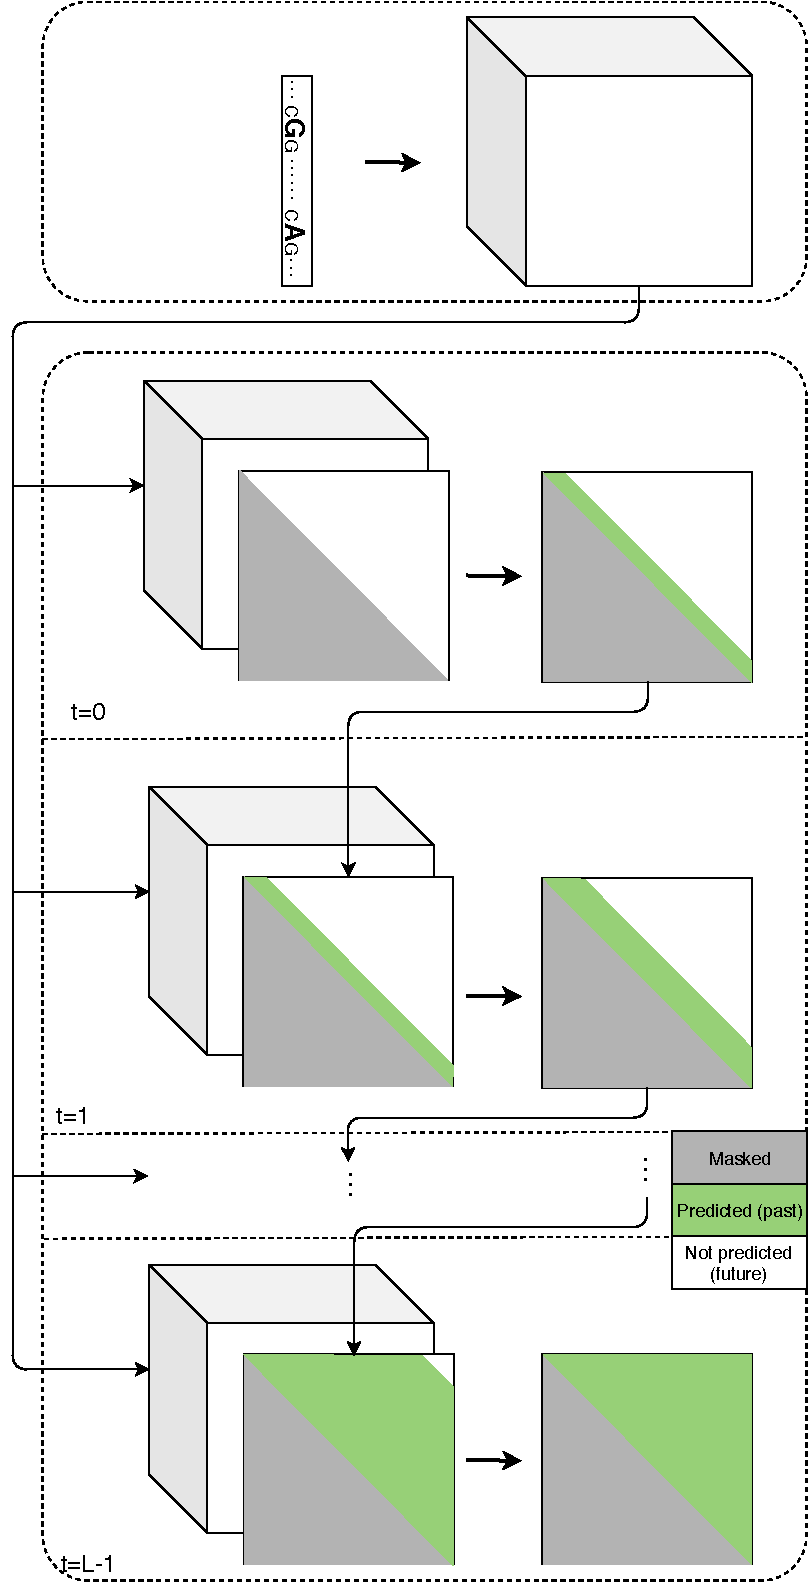
\includegraphics[width=0.4\textwidth]{plot/nn_arch_2.pdf}
        \caption{Sample structures conditioned on the input sequence.}
        \label{fig:nn_arch_2}
        \centering
%    \end{figure}
\end{wrapfigure}


%TODO plot for NN architecture

%batch, mask

\subsection{Training}

We trained the model using a synthetic dataset, constructed by sampling $50000$ random sequences with length
between $10$ and $100$.
For each sequence, we ran RNAfold\cite{lorenz2011viennarna} with the default parameters and
record the minimum free energy structure.

For each minibatch, we zero-pad the sequence array and structure matrix to the maximum length in the minibatch.
When computing the loss and gradient, entries in structure matrix that were padded are being masked,
in addition to the lower triangular entries (since we're only predicting the upper triangular matrix).

Note that although we present a single output structure for each input sequence at training time,
the model is capable of generating a distribution of structures at test time, by generalizing across different examples.

%TODO hyperparameters

%Special constraints when sampling the matrix.

%Describe dataset.

%1-step AR.


\subsection{Inference}

TODO this is repeated from the model section, maybe combine?

At test time, we can sample structures conditioned on the input sequence.
As shown in Fig \ref{fig:nn_arch_2}, we initialize the output structure with a matrix of all zeros,
then sample one slice at a time until the upper triangular matrix is filled with sampled values.
At each step, we sample a binary label for each position in the current slice based on the
Bernoulli probability predicted by the model.
To ensure the sampled structure is valid, when sampling the label for location (i, j),
if i-th or j-th position is already paired with another position (from samples in the previous timestamps),
then we set $y_{i, j}$ to $0$ without sampling from the model output.

\section{Result}

%TODO show some training performance. how?


\subsection{Test set performance}

We generated a test set with $100$ sequence, using a process similar to the training set.
Sequences are generated uniformly randomly using A,C,G,U and lengths are between $10$ and $100$.
For each sequence in the test set, we ran RNAfold (TODO more details) and sampled $100$ structures from the ensemble,
and used our model to also sample $100$ from the output distribution conditioned on the input sequence.
To avoid evaluating on low probability structures, we discarded structures that only occur once.
Then, for each unique structure produced by RNAfold, we computed sensitivity (TODO definition) and
positive predictive value (PPV, TODO definition) against all unique structures generated by our model,
and recorded the best one, where best is defined by largest ? (TODO update code + plot, since we're not using f-measure, maybe do a sum?).
This represent? how well the model recovers each of structures produced by RNAfold.
Histogram showing the distribution of these performance metric across all structures in all sequences is shown in Figure \ref{performance_test_set}.
As we can see from the figure, majority of the RNAfold-generated structures can be recovered with larger than $0.8$ sensitivity and PPV.

\begin{wrapfigure}{R}
    \centering
    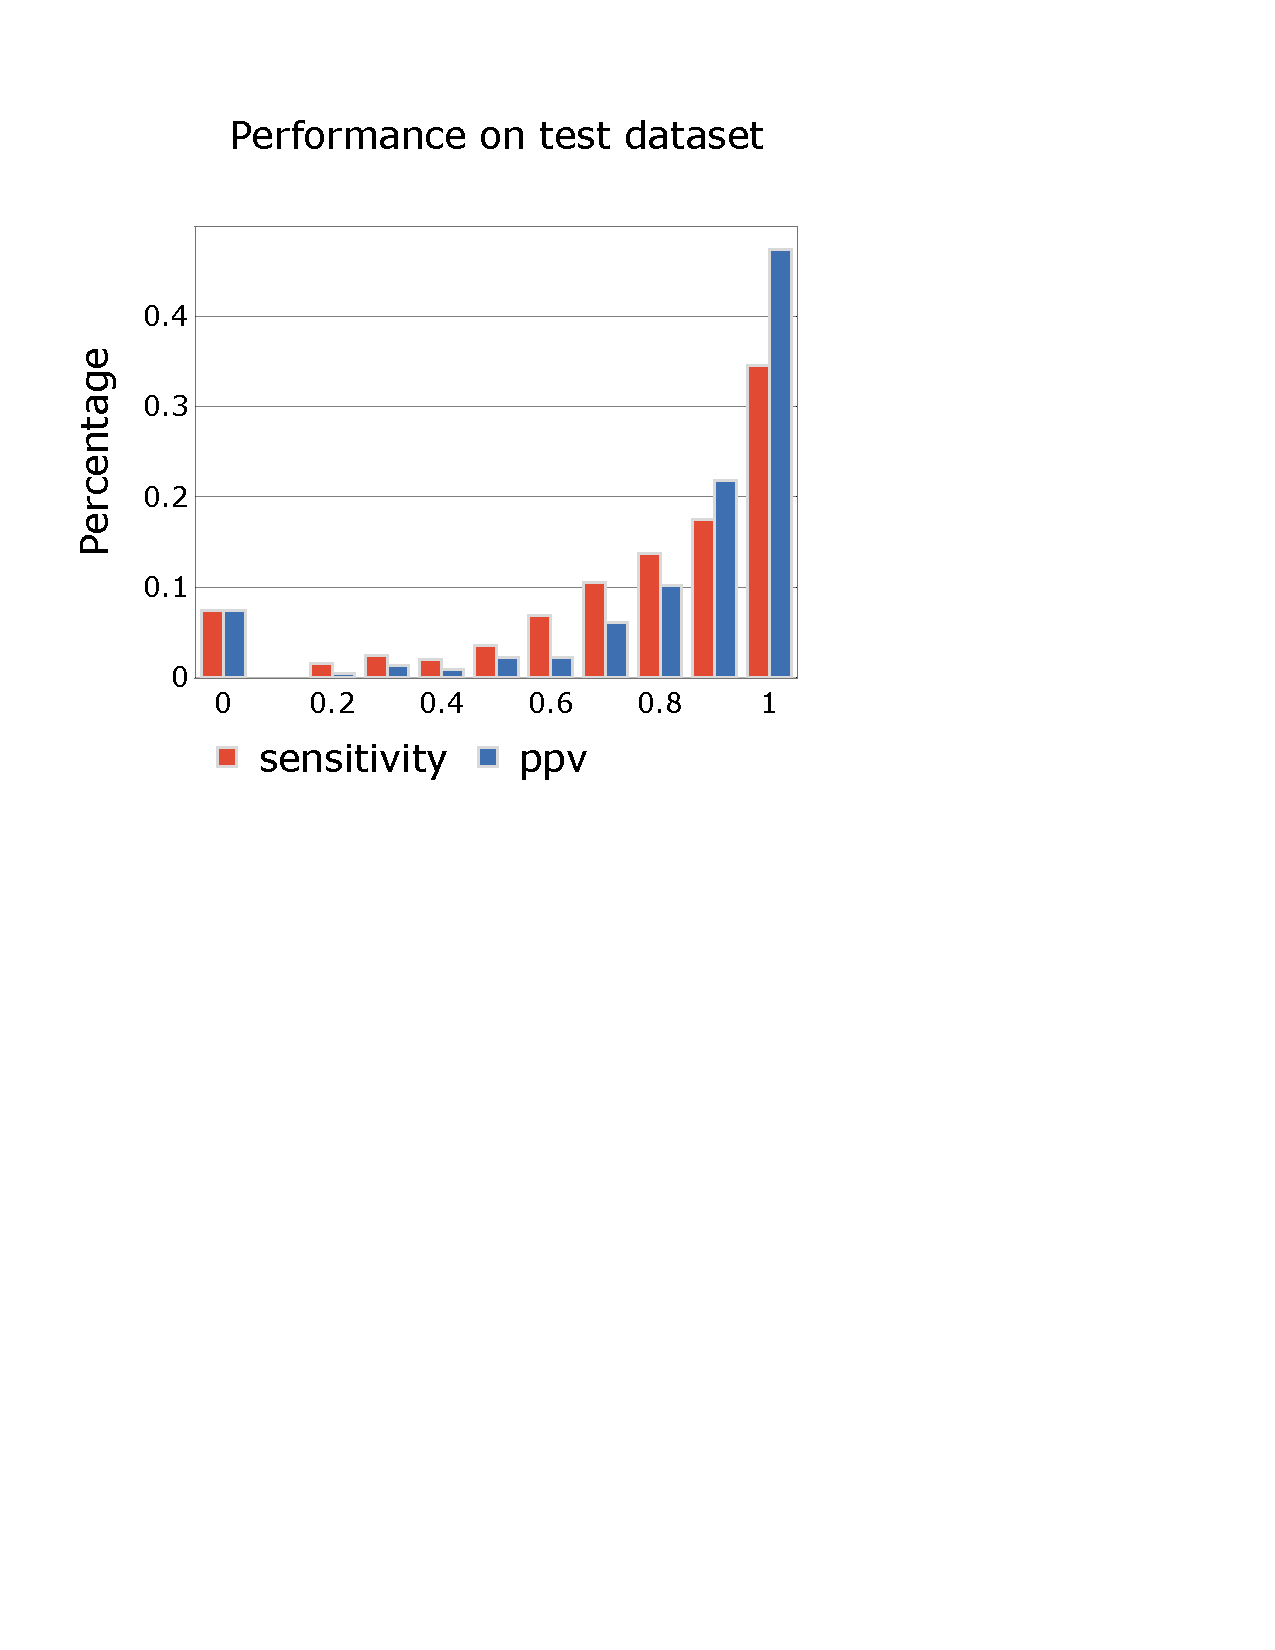
\includegraphics[width=0.4\textwidth]{plot/performance_test_set.pdf}
    \caption{TODO}
    \label{fig:performance_test_set}
    \centering
\end{wrapfigure}


% TODO run RNAfold, generate top-n strutcures in ensembl
% TODO then sample e.g. 100 structures from our model, see how frequent we can recover the ones from RNAfold

%TODO show that we can predict well-known structure.
%Any known multi-structure sequences?

%\subsection{Generate distribution of structures}
%
%As an example, for a 323-base long sequence (TODO link to DB),
%we sampled 20 structure from the model output, as shown in Fig \ref{fig:sampled_structures}.
%On the left we show the binary upper triangular matrix sampled by the model (TODO it's too tiny to see anything),
%on the right we show the corresponding secondary structure rendered as a graph (only showing 4 due to space limit).
%
%
%\begin{figure}[h!]
%    \centering
%    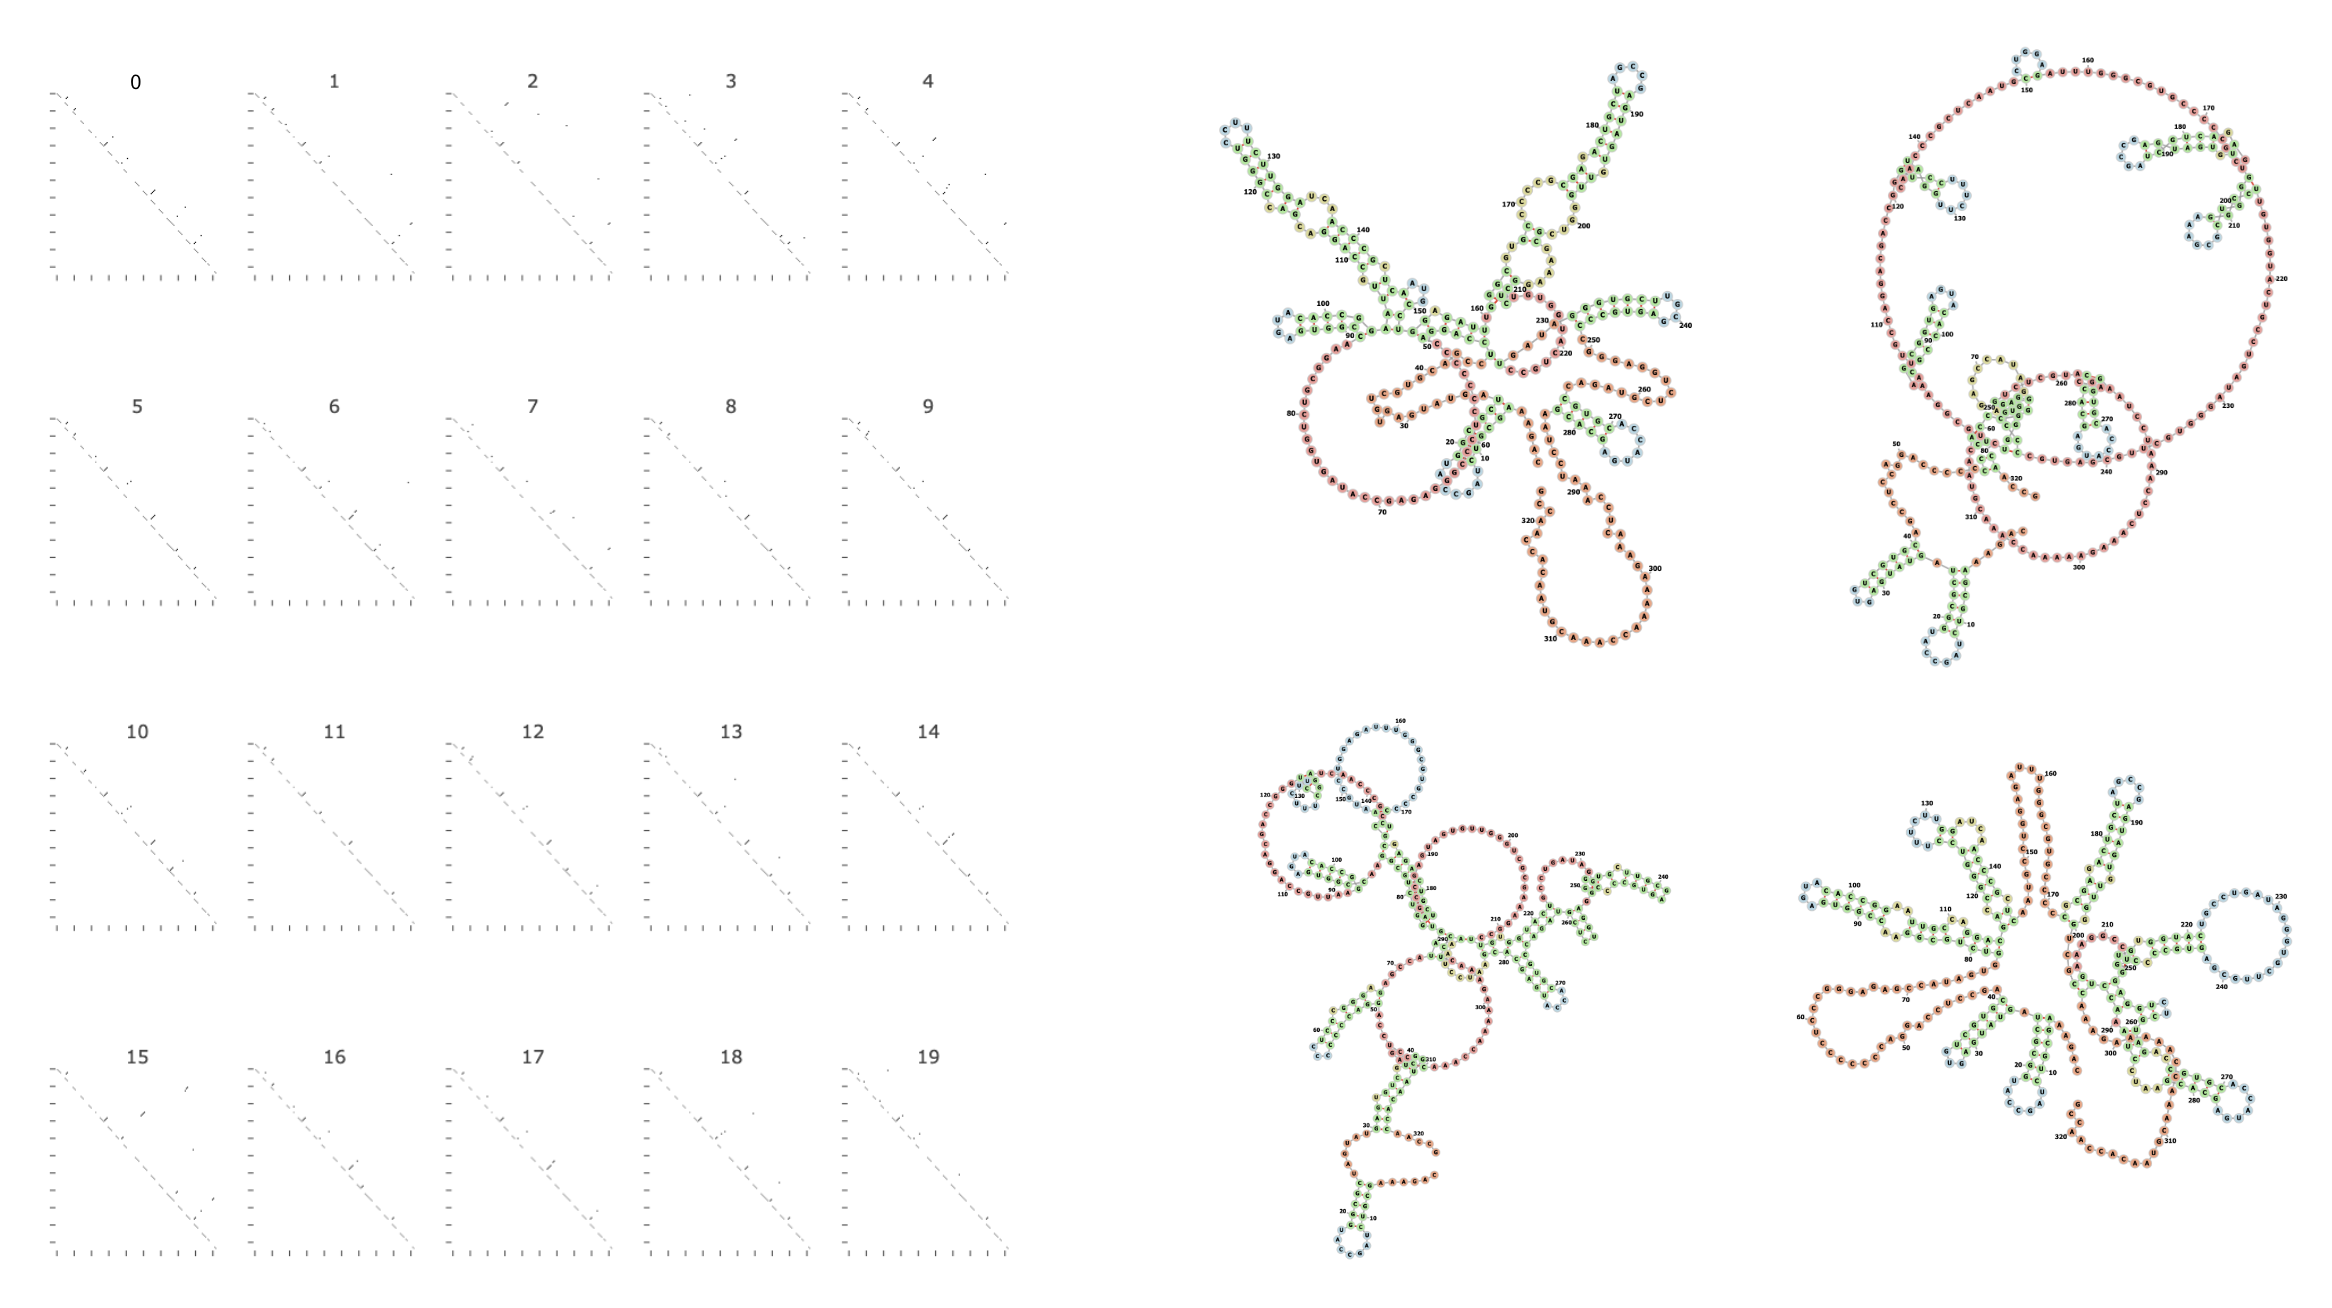
\includegraphics[width=\textwidth]{plot/sampled_structures.png}
%    \caption{TODO}
%    \label{fig:sampled_structures}
%    \centering
%\end{figure}



%TODO show generating an ensemble of structures

\subsection{Structure with pesudoknot}

Although trained on synthetic dataset with no pseudoknot structures,
since our model doesn't incorporate hard-wired rules on how local structures assemble into global structure,
it is actually capable of generating structure with pseudoknots.
As an example, we use the sequence of mouse mammary tumor virus (MMTV), whose secondary structure
contains pseudoknot as measure by nuclear magnetic resonance (NMR), as shown in Fig \ref{fig:sample_structure_pseudoknot}(a).
Minimum free energy structure predicted by RNAfold takes a quite different form, which is shown in Fig \ref{fig:sample_structure_pseudoknot}(b).
In contrast, when we sample 100 structures from our model, it shows a diverse set of possible structures,
including the one predicted by RNAfold, as shown in Fig \ref{fig:sample_structure_pseudoknot}(c3),
and more interestingly, the pseudoknot structure from NMR, as shown in Fig \ref{fig:sample_structure_pseudoknot}(c1).

%and recovered ? with knots. (TODO also show other strutures? plot? pending fixing arr2db)
%See Fig \ref{fig:sample_structure_pseudoknot}.


\begin{wrapfigure}{R}
    \centering
    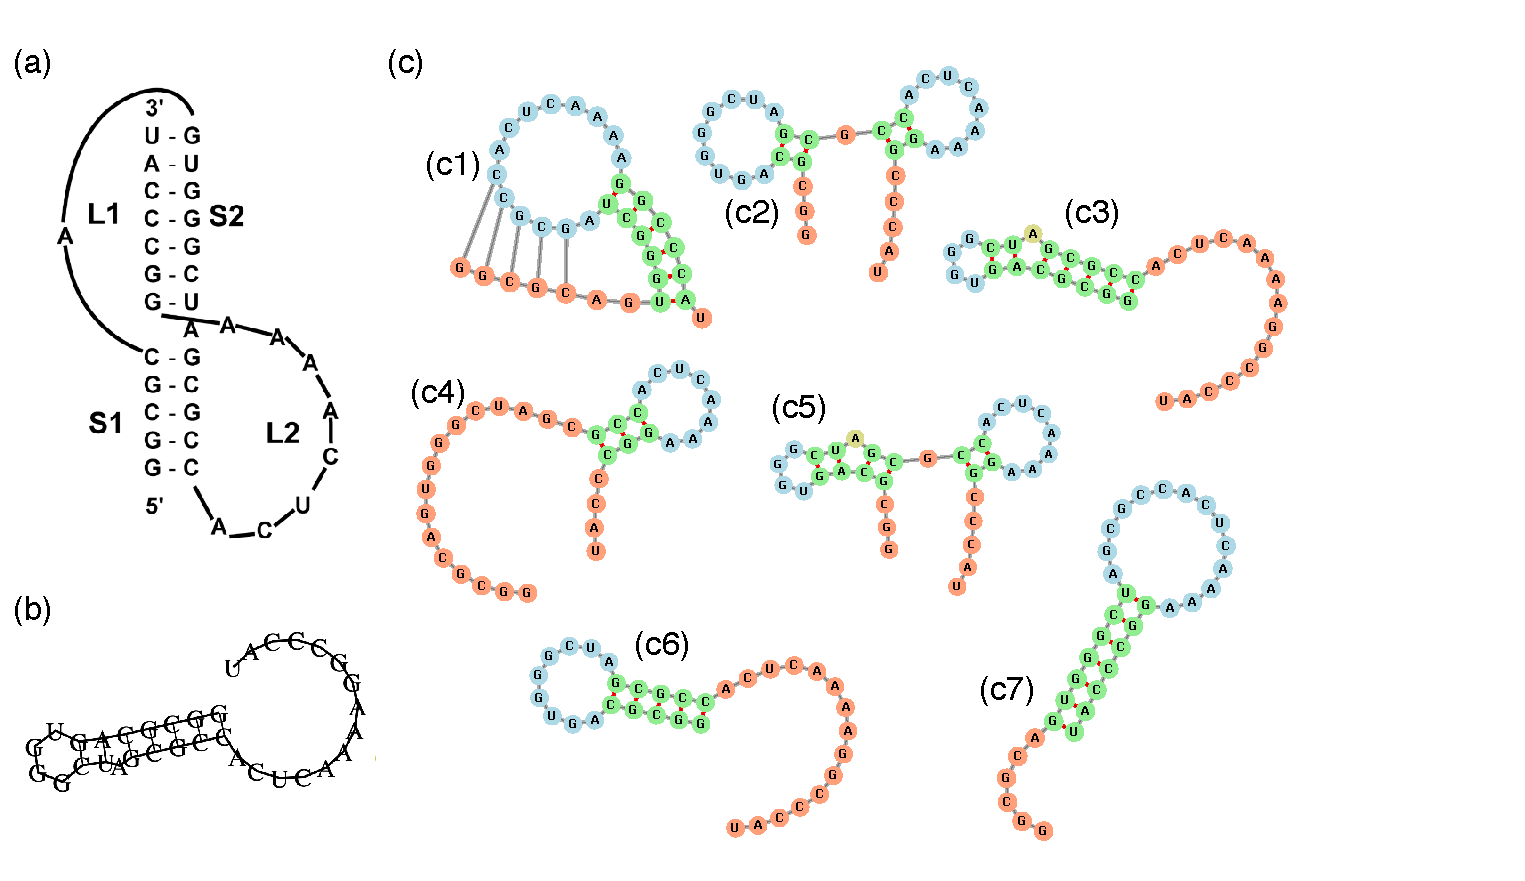
\includegraphics[width=0.8\textwidth]{plot/sample_structure_pseudoknot.pdf}
    \caption{Secondary structure of mouse mammary tumor virus (MMTV): (a) measured by nuclear magnetic resonance (NMR), plot from \cite{staple2005pseudoknots} (TODO plot was a screenshot from the paper, any problems?), (b) predicted by RNAfold web server, (c) Structures generated by our model, specifically, (c1) is a structure with pseudoknot and is identical to (a), (c3) is identical to (b).}
    \label{fig:sample_structure_pseudoknot}
    \centering
\end{wrapfigure}


%\subsection{Run time comparison}

%\subsection{Performance comparison}
%
%cross validation & test set (real sequences)
%
%\subsection{Interesting cases}

\subsection{Sequence design via gradient ascent}

One benefit of having a differentiable model like neural network is that we can answer interesting questions like:
given my current input sequence, what (small) changes can I make to maximize the pairing probability of two positions?
We illustrate this using a short RNA sequence GAUCACCUUUGGAUC.
(TODO mention sampled structures)
, with structure as shown in Fig \ref{gradient_ascent}(a).
In order to find small, local changes to be made on this sequence,
we computed the gradient of one output node $y_{i, j}$
with respect to all the input nodes ($17 \times 4$ array).
We ran $100$ gradient ascent iterations with step size $0.01$,
in each step, after adding the gradient (times step size) onto the input,
we re-normalize the input so the feature dimension sum up to 1.
Fig \ref{gradient_ascent}(b) and (c) shows the resulting sequence and structure
for $y_{5, 11}$ and $y_{6, 10}$, respectively.



\begin{wrapfigure}{R}
    \centering
    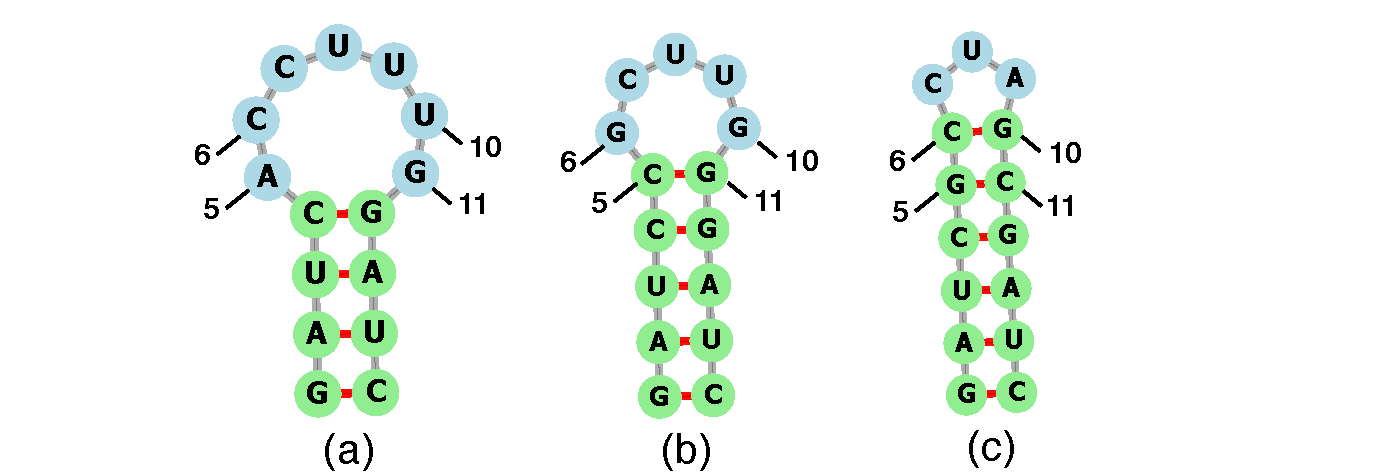
\includegraphics[width=0.4\textwidth]{plot/gradient_ascent.pdf}
    \caption{TODO}
    \label{fig:gradient_ascent}
    \centering
\end{wrapfigure}


%differentialble model. use case.

\section{Conclusion}

%future work: train on real sequences and structure (we imagine the performance will improve)
%
%different AR/sampling setup, different factorization, better performance?
%
%train on high throughput data
%
%graph nn



\clearpage

\bibliographystyle{unsrt}
\bibliography{mlcb_2019}

%Speed consideration: implement split architecture, only need one forward pass for up to the last layer,
%then run last layer (triangular convolution) for $L-1$ times.
%
%
%Case study:
%
%TODO compare with RNAfold performance


\end{document}
